\documentclass[11pt,a4paper]{report}
\usepackage[margin=0.5in]{geometry}
\usepackage[explicit]{titlesec}
\usepackage[dvipsnames]{color}
\usepackage{graphicx}
\usepackage{alltt}

\definecolor{mygray}{gray}{.75}

\titleformat{name=\section,numberless}[display]
  {\normalfont\scshape\Large}
  {\hspace*{-10pt}#1}
  {-15pt}
  {\hspace*{-110pt}\rule{\dimexpr\textwidth+80pt\relax}{2pt}\Huge}
\titlespacing*{\section}{0pt}{30pt}{10pt}

\titleformat{name=\subsection,numberless}[display]
  {\normalfont\scshape}
  {\hspace*{-10pt}#1}
  {-15pt}
  {\hspace*{-110pt}\rule{\dimexpr\textwidth+30pt\relax}{0.4pt}\Huge}
\titlespacing*{\subsection}{0pt}{20pt}{5pt}


\begin{document}

\noindent\Large\textbf{CM2303 (Algorithms \& Data Structures)}\\
\noindent\large\textit{Non-assessed Labs}
\vskip30pt

\section*{Lab 2.3: Traversing Trees}

In Lab 2.2 we used trees as a way for storing hierarchical data. However, trees are only useful for storing data if it can also be retrieved later. Querying trees for data is done using tree \textit{traversal}, and there are multiple ways in which this can be done. The two most common traversals use stacks and queues to store subsets of visited nodes.

The questions in this exercise require your tree implementation from Lab 2.2. If you haven't yet completed that exercise then please do so before continuing. 

\begin{enumerate}

\item A \textit{queue} is a data structure that supports the `first in, first out' mantra. \\
    \begin{center}
        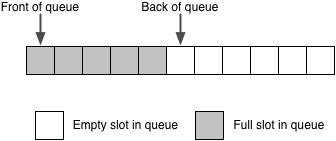
\includegraphics[width=.4\textwidth]{media/queue.png} \\
    \end{center}
    New elements are added to the back of the queue and elements are retrieved from the front of the queue.\\
    \vskip5pt
    Write a Java class, called \texttt{Queue}, that implements a queue for objects of type \texttt{Node} using inbuilt Java collection classes (such as arrays or lists). Your class should include the following methods:
    \begin{itemize}
        \item \texttt{enqueue(Node node)} - Add a new \texttt{Node} object to the queue.
        \item \texttt{dequeue()} - Retrieve and remove a \texttt{Node} object from the queue.
        \item \texttt{is\_empty()} - Returns \texttt{true} if queue is empty, and \texttt{false} if otherwise.
    \end{itemize}
 
\item A \textit{stack} is a data structure that supports the `first in, last out' mantra. \\
    \begin{center}
        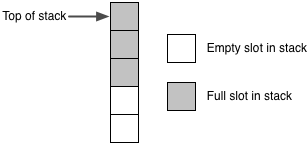
\includegraphics[width=.4\textwidth]{media/stack.png} \\
    \end{center}
    New elements are added to the top of the stack and elements are also retrieved from the top of the stack.\\
    \vskip5pt
    Write a Java class, called \texttt{Stack}, that implements a stack for objects of type \texttt{Node} using inbuilt Java collection classes (such as arrays or lists). Your class should include the following methods:
    \begin{itemize}
        \item \texttt{push(Node node)} - Add a new \texttt{Node} object to the stack.
        \item \texttt{pop()} - Retrieve and remove a \texttt{Node} object from the stack.
        \item \texttt{is\_empty()} - Returns \texttt{true} if stack is empty, and \texttt{false} if otherwise.
    \end{itemize}

\item Write a method for your \texttt{Tree} class called \texttt{breadth\_first\_search()} that accepts a single integer: the ID of the \texttt{Node} object from which to start a breadth-first traversal of the tree. Implement this method using the outline pseudocode below (adapted from that provided in lectures):
\begin{alltt}
Add start node to queue
while length of queue > 0:
    Retrieve a node from the queue
    Add all children of the node to the queue
\end{alltt}
    Modify your method so that it prints out the ID of every node it `visits' on one line, separated by spaces.

\item Write a method for your \texttt{Tree} class called \texttt{depth\_first\_search()} that accepts a single integer: the ID of the \texttt{Node} object from which to start a depth-first traversal of the tree. Implement this method using the outline pseudocode below (adapted from that provided in lectures):
\begin{alltt}
Add start node to stack
while length of stack > 0:
    Retrieve a node from the stack
    Add all children of the node to the stack
\end{alltt}
    Modify your method so that it prints out the ID of every node it `visits' on one line, separated by spaces. 

\item Using your \texttt{Tree}'s \texttt{add\_node()} method, create an instance of \texttt{Tree} that represents the following hierarchy:
    \begin{center}
        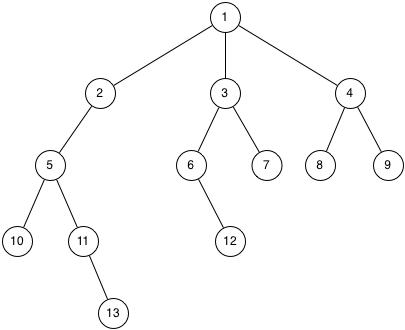
\includegraphics[width=.6\textwidth]{media/tree.png}
    \end{center}

\item Traverse your tree object using your \texttt{breadth\_first\_search()} and \texttt{depth\_first\_search()} methods starting from node 1. Verify that the output of these methods looks something like the below. \textit{(hint: you may need to insert a new line between the output of both methods).}
\begin{verbatim}
$ javac TreeTraversal.java
$ java TreeTraversal
1 2 3 4 5 6 7 8 9 10 11 12 13
1 4 9 8 3 7 6 12 2 5 11 13 10
\end{verbatim}

The first line of output represents breadth-first traversal and the second line is depth-first. Don't worry if your output for depth-first goes from right-to-left (as in the example above) - the key is that branches are fully explored one at a time. 

\item Modify your search methods so that they are both of return type \texttt{Node} and that they accept a second integer argument. If this new argument is non-\texttt{null}, it represents the ID of a node to search for. If the node is found, it should be returned at the point it is `visited'. If the whole tree is traversed without finding the node, then the methods should return \texttt{null}. If the second argument is \texttt{null}, then the tree should just be traversed as before (though it will still need to return a \texttt{null} value).

\item Use breadth-first search to find nodes 2 and 12. Verify that it is much quicker to find node 2 than 12 by checking that the method visits fewer nodes.

\item Use depth-first search to find find the same nodes. Verify that it is quicker to find node 12 than node 2, despite node 2 being closer to the root node.

\item \textbf{Non-essential question}\\
        Implement \textit{depth-limited searching} in your \texttt{Tree} class. For this, you will need to create two new methods, as described in the lecture notes. One method to carry out the depth-first search at a particular depth and the second to gradually increase the depth until the node is found. Depth-limited searching reduces the required size of the stack, and therefore reduces the memory load of the operation.

        Pseudocode for this procedure is provided in your lecture notes.


\end{enumerate}

\end{document}
